\documentclass[11pt, letterpaper,titlepage,oneside]{article}
\usepackage[margin=1in]{geometry}
\usepackage{titlesec}
\usepackage{fancyhdr}
\fancyhf{}
\renewcommand{\headrulewidth}{0pt}
\rfoot{\thepage}
\pagestyle{fancy}
%paragraph indentation
\usepackage[parfill]{parskip}
\parskip = \baselineskip
\setlength{\parindent}{0in}
\usepackage{xcolor,graphicx}
\usepackage{float}
\usepackage{amsmath}
\usepackage[T1]{fontenc}
\usepackage{mathptmx}
\usepackage{lipsum}
\renewcommand{\arraystretch}{1}
% Caption Formatting
\usepackage{caption}
\captionsetup[figure]{labelsep=period}
\captionsetup[table]{labelsep=newline, justification=centering}
\renewcommand{\tablename}{TABLE}
\renewcommand{\thetable}{\Roman{table}}
\usepackage{fixltx2e}
\usepackage{listings}

%Script font
\usepackage[mathscr]{euscript}
\renewcommand{\thesection}{\Roman{section}.}
\renewcommand{\thesubsection}{\thesection\Alph{subsection}.}
\renewcommand{\thesubsubsection}{\thesection\Alph{subsection}.\arabic{subsubsection}}

\begin{document}


\begin{center}
\Large{\textbf{Load Balancing by Dimension}}
\end{center}
\bigskip

\section*{Introduction}

As has been proven over the last few months, we need an improved load balancing algorithm. The most popular option that can be implemented in PDT now is the now-called Load Balancing by Dimension (LBD) algorithm. The gist of the algorithm is to first move X cut planes and use the column wise load balance metric, $f_I$, to determine when to stop redistribution, and then to load balance each row WITHIN each column. 

This will of course lead to a major issue: the determination of each subset's neighbor is no longer as easy. Previously, we were able to use a simple $i,j$ indexing for each subset, which makes the determination of neighbors trivial. Now, with cut planes in Y no longer lining up perfectly, a subset can have mutiple neighbors to the right or left, not just one of each. Figure \ref{initial} shows the $i,j$ functionality, while Fig. \ref{now} shows the current predicament. 

\begin{figure}[H]
\centering
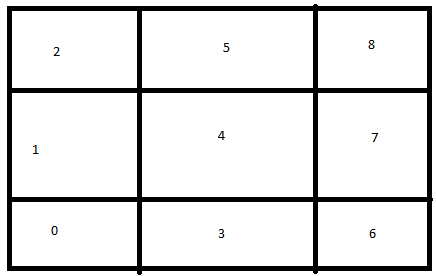
\includegraphics{Initial.png}
\caption{The previous load balancing algorithm result that allows for the $i,j$ system of determining the four neighbors for each subset. Numbers are subset IDs.}
\label{initial}
\end{figure}

\begin{figure}[H]
\centering
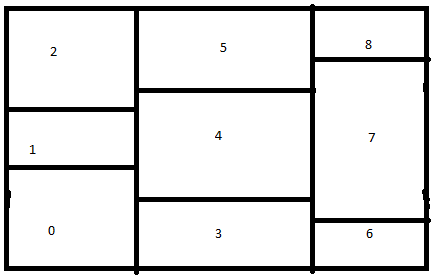
\includegraphics{Now.png}
\caption{A load balancing by dimension example result that disallows the use of the $i,j$ system of determining neighbors. Numbers are subset IDs.}
\label{now}
\end{figure}

\newpage
\section*{Pseudocode}

\lstinputlisting[language = C++, basicstyle = \footnotesize, breaklines=true,numbers = left,stepnumber=5,firstnumber=1,numberfirstline=true]{load_balance_by_dimension.cc}

\newpage
\section*{Examples}

Let's look at Fig. \ref{now} once more.

\begin{figure}[H]
\centering
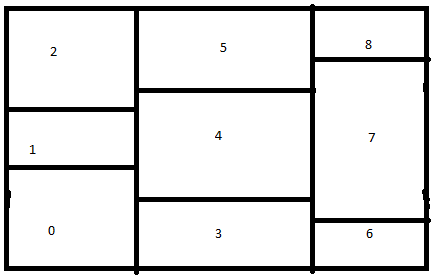
\includegraphics{Now.png}
\caption{A load balancing by dimension example result that disallows the use of the $i,j$ system of determining neighbors. Numbers are subset IDs.}
\label{now}
\end{figure}

Let's take a look at subset 0 and follow through the pseudocode in the BUILD\_UNDIRECTED\_GRAPH function (line 42) :

\begin{itemize}
\item Subset 0 is located in the first column, so it's only potential neighbors are to the right in the second column.
\item We pull the cut line information for the second column, and we look at the two cut interior cut lines, not the cut lines on the global boundary.
\item Looking at the first cut line in the second column, we see that it is less than subset 0's y-max, and greater than subset 0's y-min. Therefore, the two subsets that share this cut line as a boundary, subsets 3 and 4, are added as neighbors to subset 0. 
\item Looking at the second cut line in the second column, we see that it is above subset 0's y-max, so we check that the previous cut line is below subset 0's ymax. It is, so subset 4 is added as a neighbor again.
\item Duplicates are removed, and subsets 3 and 4 are subset 0's neighbors to the right/left.
\end{itemize}

We take a look at subset 4 and follow through the pseudocode in the same way:

\begin{itemize}
\item Subset 4 is not located in the first or last column, so it's potential neighbors are in the columns to the left and right.
\item  We pull the cut line information for the right and left columns, and we look at the two cut interior cut lines, not the cut lines on the global boundary.
\item Looking at the first cut line in the left column, we see that it is less than subset 4's ymax, and greater than subset 4's ymin. Therefore, the two subsets that share this cut line as a boundary, subsets 0 and 1, are added as neighbors to subset 4.
\item Looking at the second cut line in the left column,  we see that it is less than subset 4's ymax, and greater than subset 4's ymin. Therefore, the two subsets that share this cut line as a boundary, subsets 1 and 2, are added as neighbors to subset 4.
\item Looking at the first cut line in the right column, we see that it is less than subset 4's ymax, and less than subset 4's ymin. No neighbor is added.
\item Looking at the second cut line in the right column, we see that it is greater than subset 4's ymax. The previous cut line is less than subset 4's ymax, so the subset that has the second cut line as its ymax, subset 7, is added as a neighbor to subset 4.
\item Duplicates are removed, and subsets 0,1,2, and 7 are subset 4's neighbors to the right/left.
\end{itemize}


\end{document}